\documentclass[12pt,a4paper]{article}
% \usepackage[english]{babel}
% \usepackage[utf8x]{inputenc}
\usepackage[export]{adjustbox}

\usepackage{graphicx} % Required for inserting images.
\usepackage[margin=25mm]{geometry}
\parskip 4.2pt  % Sets spacing between paragraphs.
% \renewcommand{\baselinestretch}{1.5}  % Uncomment for 1.5 spacing between lines.
\parindent 8.4pt  % Sets leading space for paragraphs.
\usepackage[font=sf]{caption} % Changes font of captions.

\usepackage{amsmath}
\usepackage{amsfonts}
\usepackage{amssymb}
\usepackage{siunitx}
\usepackage{verbatim}
\usepackage{hyperref} % Required for inserting clickable links.
\usepackage{natbib} % Required for APA-style citations.


\title{Motion planning for Nonholonomic Vehicles}
\author{Shambhuraj Anil Mane}

\begin{document}
\maketitle

\begin{abstract}
    This report presents the results of implementing a kinematic path planner to park three vehicles of increasing complexity into a tight space. The vehicles - a delivery robot, car, and truck with trailer - each have different steering constraints. A simulated 2D environment was created with obstacles, and configurations space was modeled accounting for nonholonomic constraints. Custom path planning algorithms generated feasible paths satisfying kinodynamic constraints to maneuver each vehicle from a start position into the target parking spot. The planned paths are presented along with snapshots visualizing the parking maneuvers. Though simplistic, this project demonstrates automated parking for nonholonomic vehicles in cluttered environments.
\end{abstract}

\begin{figure}[htbp!]
\begin{center}
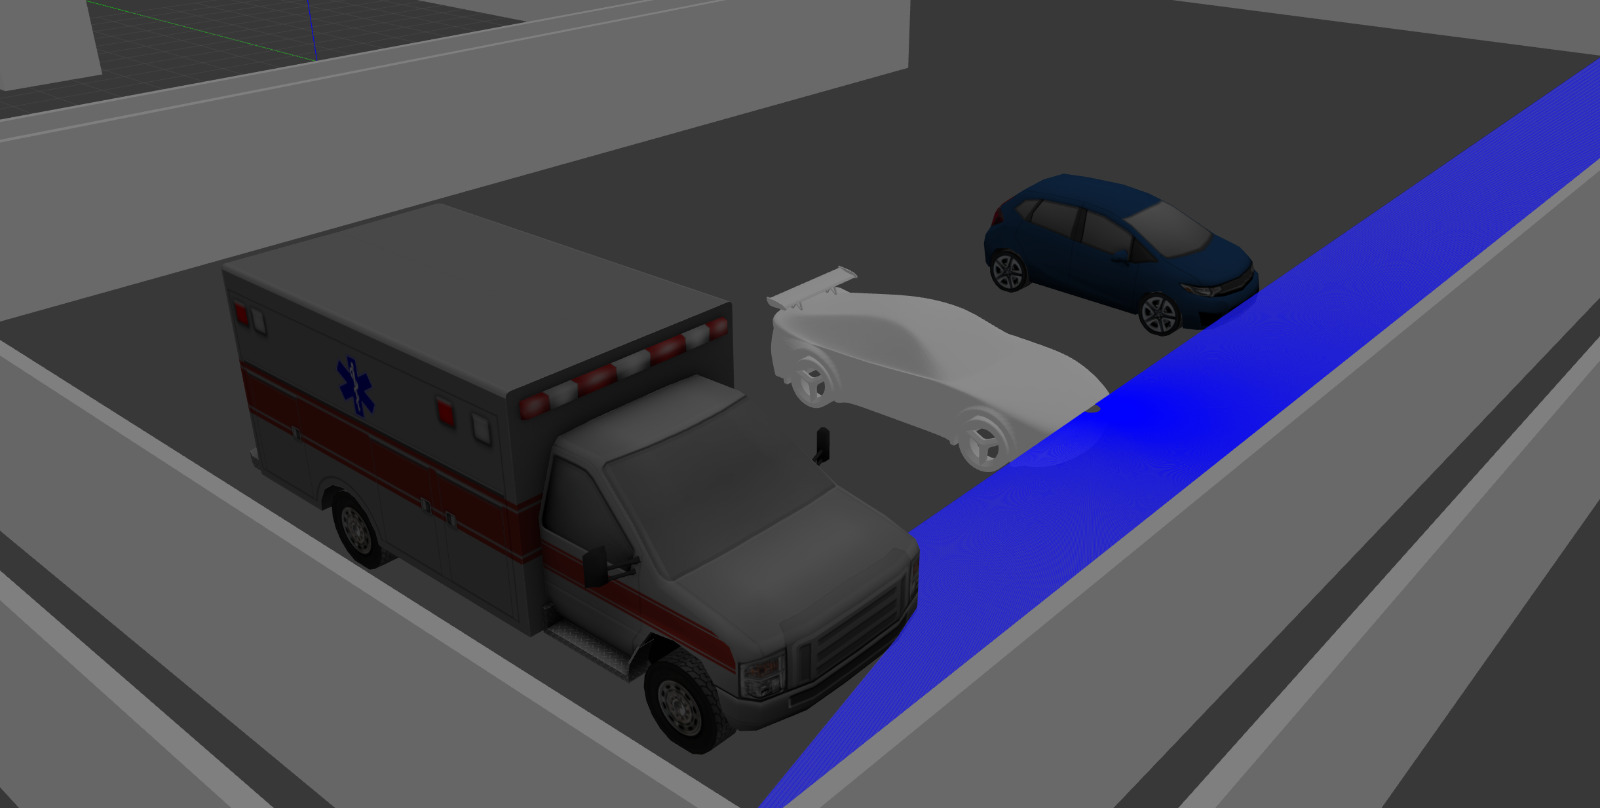
\includegraphics[width=1.0 \columnwidth]{images/park.jpeg}
\end{center}
\caption{Autonomous Parking Simulation }
\label{fig:Occupancy_grid}
\end{figure}
\pagebreak
\section{Introduction}\label{sec:intro}
This project involves developing path planning algorithms to park vehicles in a cluttered environment. The objective is to maneuver three vehicles - each with different steering constraints - from a start position to a tight parking spot, while avoiding collisions. This is a common challenge faced by autonomous vehicles operating in urban environments.\par
The simulated 2D world consists of a parking lot with obstacles flanking the target parking space on two sides. Additionally, there are multiple obstruction in the middle of the lot. The vehicles must navigate around these obstacles and utilize their full range of steering motion to efficiently park in the compact spot.\par

The three vehicles of increasing complexity are:
\begin{itemize}
    \item Delivery robot: Differential drive/skid steering
    \item Car: Ackermann steering
    \item Truck with trailer: Ackermann steering plus trailer kinematics 
\end{itemize}
Each vehicle has kinodynamic constraints in the form of nonholonomic constraints dictated by its steering mechanism. The path planner utilizes a hybrid A* algorithm which takes into account these constraints to generate feasible trajectories.\par

This project demonstrates automated parking for vehicles with different steering configurations in a constrained space using a custom motion planning algorithm.\par
\begin{figure}[htbp!]
\begin{center}
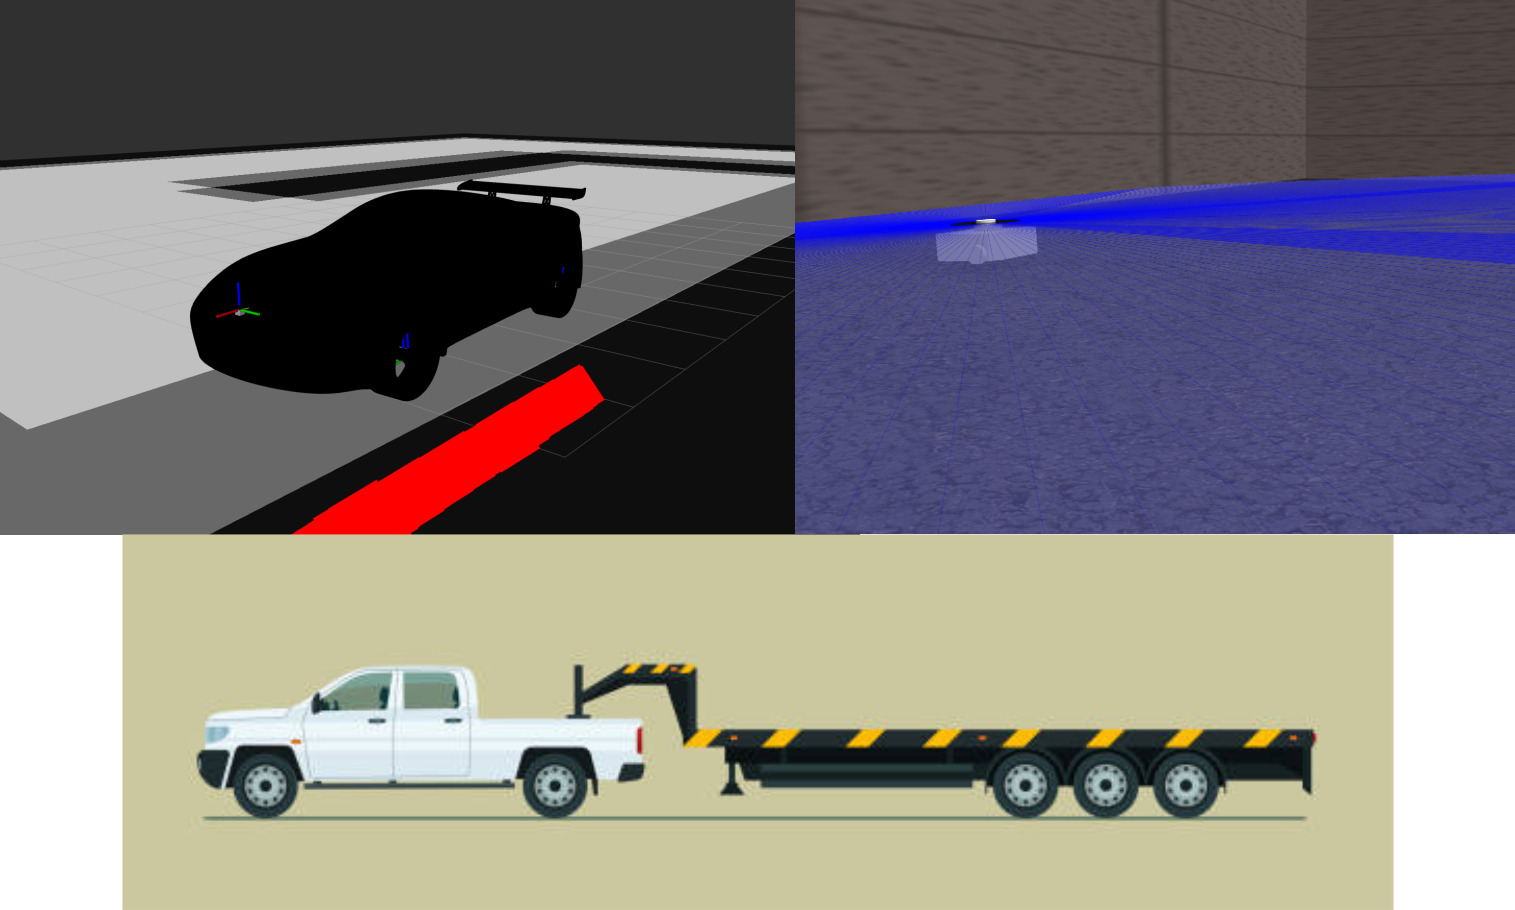
\includegraphics[width=1.0 \columnwidth]{images/3_models.jpeg}
\end{center}
\caption{Three types of Vehicles}
\label{fig:Occupancy_grid}
\end{figure}
\pagebreak



\section{Methods}\label{sec:methods}

The path planning approach taken involves using a hybrid A* search algorithm to generate optimal trajectories for parking each vehicle. This extends the traditional A* graph search by incorporating kinodynamic constraints in the cost function.

\begin{itemize}
    \item Simulation \par 
The complete parking scenario was simulated using pyplot as well as ROS2 and Gazebo. Pyplot provided ease in visualizing and working on algorithms in 2D environment and ROS2 provided the infrastructure for controlling the vehicles and visualizing the environment. Gazebo handled the physics simulation and rendering.
\par

    \item Collision Checking \par 
Continuous spaces are mathematically challenging to work with, especially when planning paths and performing collision checks. Discretizing the space simplifies the problem by dividing it into smaller, manageable states. It allows the algorithm to check for collisions with obstacles by examining a finite number of states, rather than continuously evaluating the entire continuous space.
\par

    \item Discrete Motion Planning with Nonholonomic Constraints \par 
Kinodynamic planning is crucial for vehicles and robots with non-holonomic constraints, such as cars, or robots with differential drive systems. These systems cannot instantly change their velocity or direction and have specific dynamics that must be considered to plan feasible trajectories. The diagram and explanation on this topic is given in the appendix section.
\par

    \item Hybrid A-star algorithm \par 
The path planning approach taken involves use of a hybrid A* search algorithm to generate optimal trajectories for parking each vehicle. This extends the traditional A* graph search by incorporating kinodynamic constraints in the cost function.

At each iteration, the algorithm considers reachable configurations based on the vehicle's kinematics. It selects the lowest cost node based on the A* evaluation function: f(n) = g(n) + h(n). The function g(n) represents the path cost from start to node n, while h(n) estimates the cost to reach the goal. The kinodynamic constraints are encoded in g(n) to prune infeasible motions.

This process repeats, expanding nodes until the goal is reached. The optimal path minimizing traversal cost while satisfying steering constraints is then extracted. This path is converted to a time-parameterized trajectory using the kinematic model.
\par

\end{itemize}




The complete scenario is simulated in matplotlib and ROS2 with Gazebo managing the physics and visualizing the environment.


\pagebreak
\section{Results}\label{sec:result}
The hybrid A* path planner successfully generated collision-free trajectories to park all three vehicles in the allotted space.

For the delivery robot, a smooth path was produced utilizing the differential drive constraints to neatly maneuver around the obstacles to the goal position. The planned path is shown in Figure overlaid on the environment map.

The sedan also navigated the cluttered parking lot efficiently as seen in Figure. The Ackermann steering constraints resulted in wider turns compared to the delivery robot.

Parking the truck with trailer was most challenging due to the trailer kinematics. The planner accounted for these constraints and planned a feasible path to the goal as shown in Figure. Executing the maneuver required careful tuning of velocities and accelerations.

All vehicles managed to avoid collisions and navigate within their steering limitations. 

\begin{figure}[htbp!]
\begin{center}
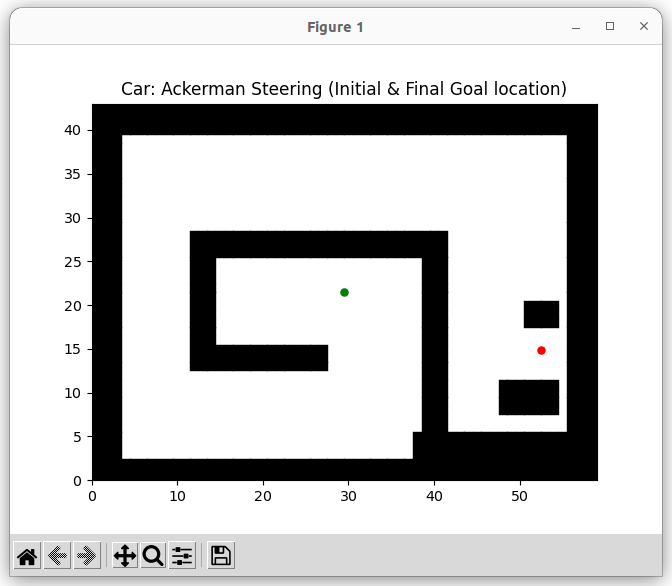
\includegraphics[width=0.3 \columnwidth]{results/car/Car-goal_setting.png}
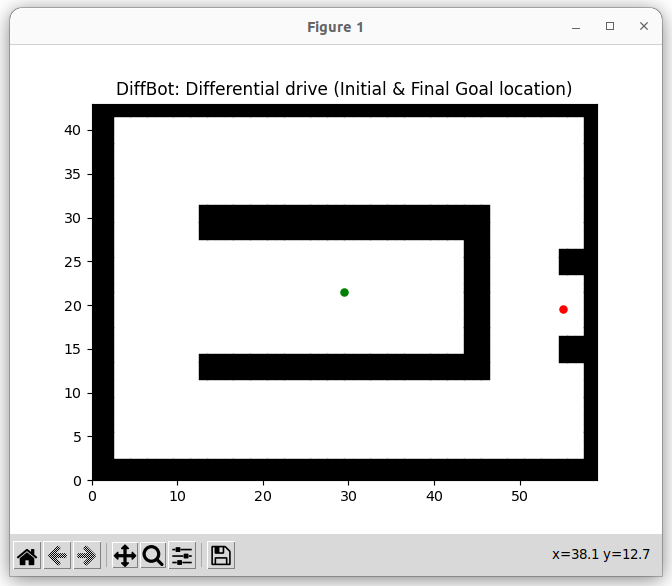
\includegraphics[width=0.3 \columnwidth]{results/diffbot/diffbot_goal_setting.png}
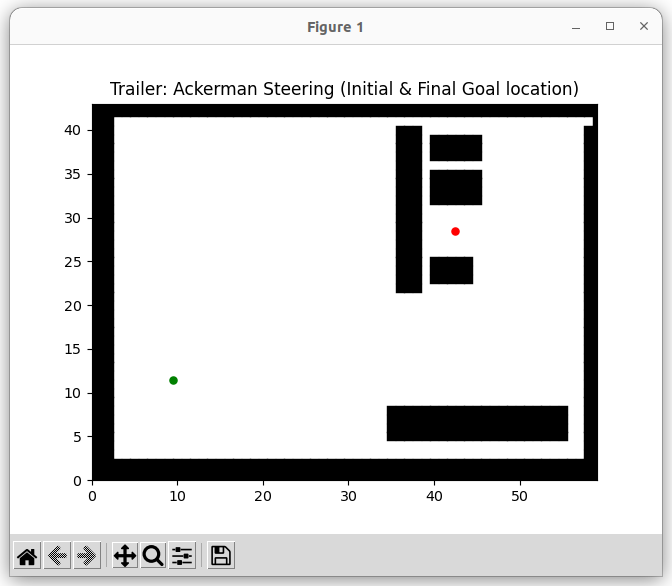
\includegraphics[width=0.3 \columnwidth]{results/truck/Truck-goal_setting.png}

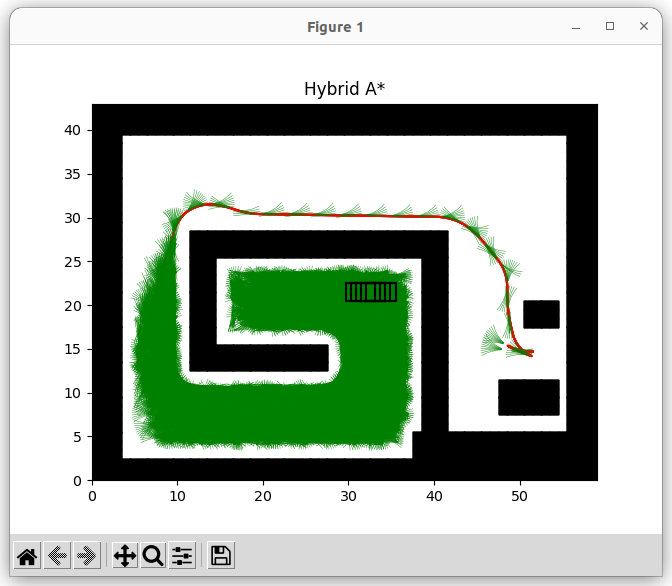
\includegraphics[width=0.3 \columnwidth]{results/car/motion_priomitives.png}
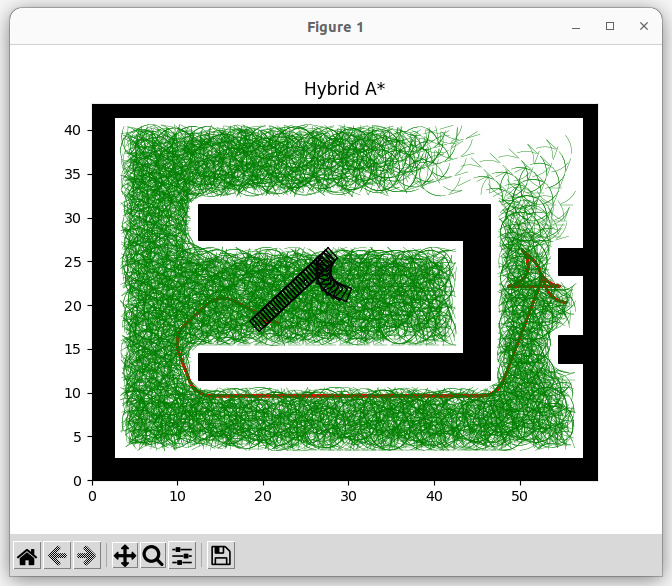
\includegraphics[width=0.3 \columnwidth]{results/diffbot/diff_motion_primitive.jpeg}
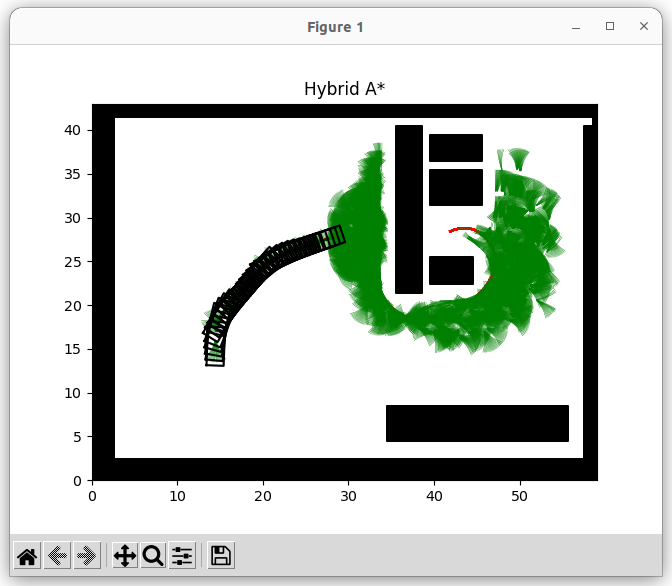
\includegraphics[width=0.3 \columnwidth]{results/truck/motion_prim.png}


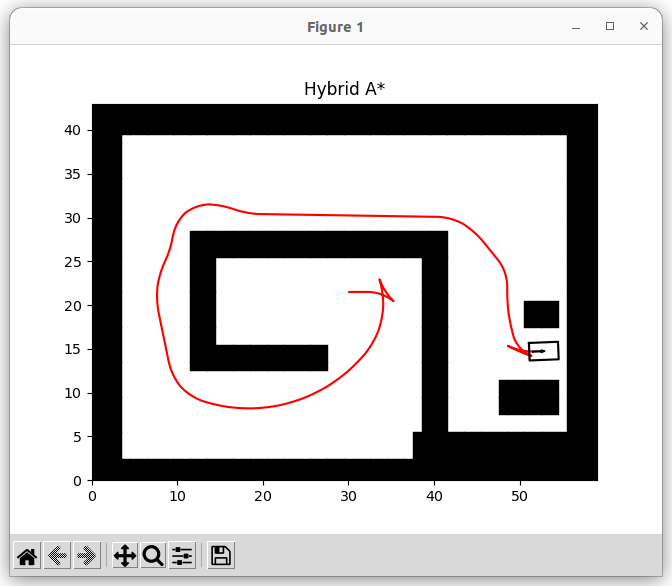
\includegraphics[width=0.3 \columnwidth]{results/car/Car-planned_path.png}
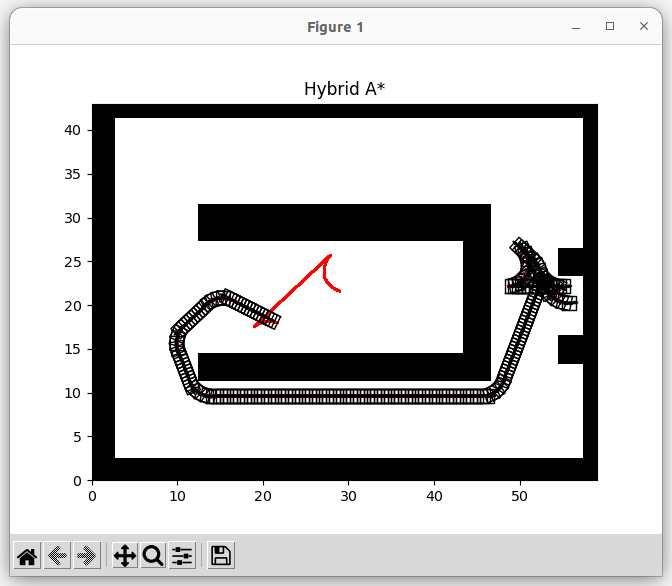
\includegraphics[width=0.3 \columnwidth]{results/diffbot/diffbot_planned_path.jpeg}
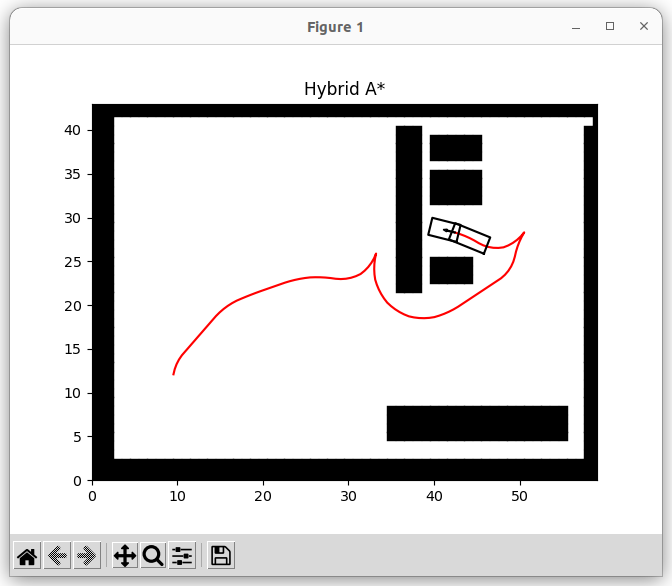
\includegraphics[width=0.3 \columnwidth]{results/truck/Truck-Planned_path.png}



\end{center}
\caption{Planned path in all three scenarios}
\label{fig:Occupancy_grid}
\end{figure}

Cost functions have been instrumental in the path planning process. Even minor alterations in their values have had a significant impact on factors such as path length, exploration duration, and the number of directional changes.

The incorporation of heuristic costs effectively reduced exploration time, enabling the path to converge to the goal point more swiftly. However, it's worth noting that the resulting path, while expedited, may not always be optimal in terms of both length and directional adjustments. On the other hand, when the heuristic cost is disregarded (hybridCost=0), it leads to more extensive space exploration, resulting in prolonged exploration times. Nevertheless, this approach tends to yield an optimized path in both length and directional adjustments. The following figures serve as conclusive evidence of the outcomes described above.
\begin{figure}[htbp!]
\begin{center}
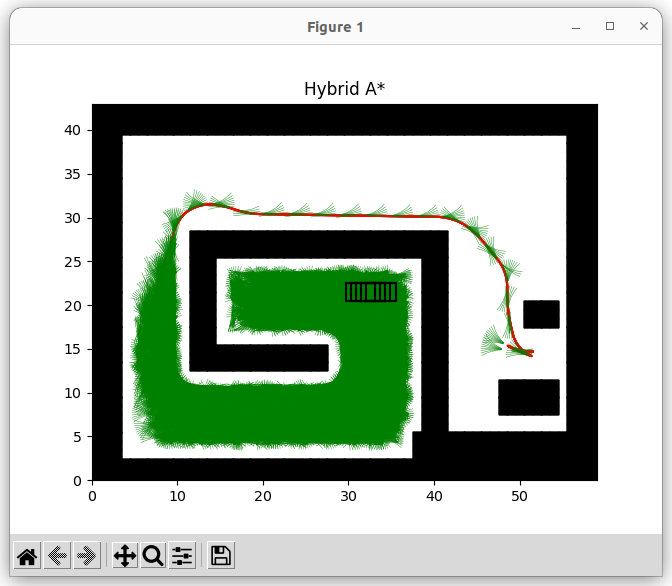
\includegraphics[width=0.4 \columnwidth]{results/car/motion_priomitives.png}
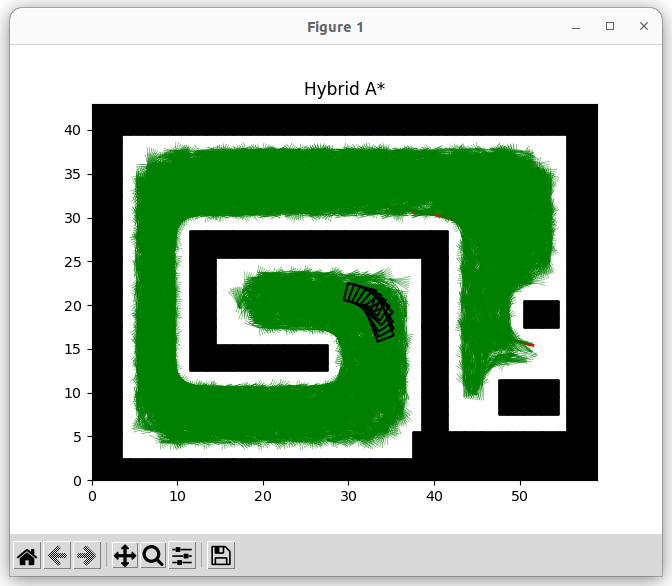
\includegraphics[width=0.4 \columnwidth]{results/car/without_heuritic.png}
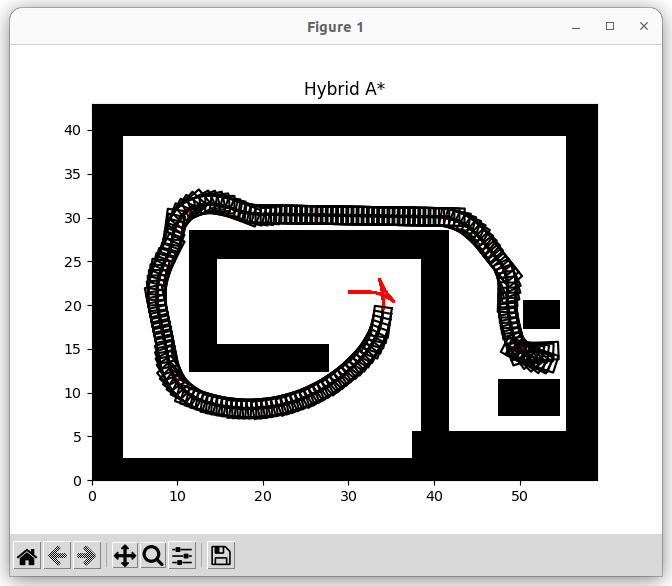
\includegraphics[width=0.4 \columnwidth]{results/car/path-with heuritic.png}
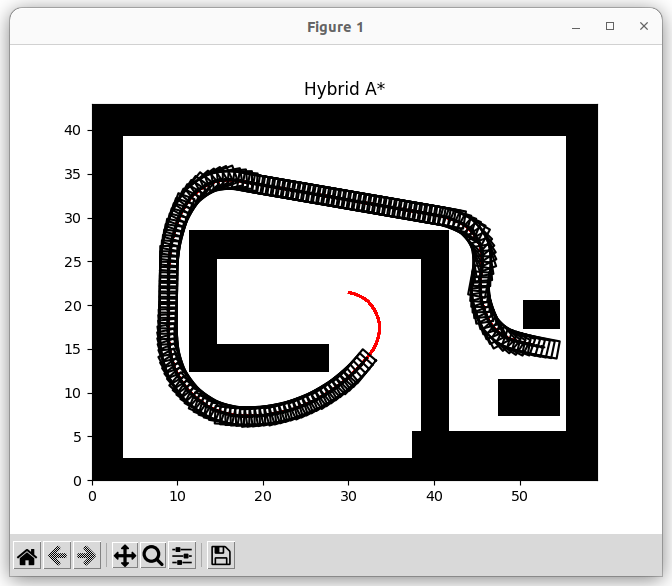
\includegraphics[width=0.4 \columnwidth]{results/car/path_without_heuristic.png}

\end{center}
\caption{Path length and explored states comparison}
\label{fig:Occupancy_grid}
\end{figure}

\section{Conclusion}\label{sec:discussion}

This project demonstrated successful path planning and control of various steered vehicles for parking in tight spaces. Optimal, collision-free trajectories were generated taking into account kinodynamic constraints of each vehicle model.

The hybrid A* motion planning algorithm was effective at producing smooth paths to the goal in reasonable time. On average, parking was completed within 20-35 seconds for the vehicles. The planner balances exploration of the configuration space with exploitation of lowest cost paths. Further tuning of heuristic functions could improve planning times.

While the planned paths were optimal in terms of length, the trajectories could be further optimized for time. Velocity profiles could be smoothed to minimize accelerations and jerks. Dynamic constraints could also be incorporated within the kinodynamic framework to generate time-optimal trajectories.

The system could be extended to more complex vehicles, tighter environments, and dynamic obstacles. Overall, this project demonstrated automated parking for nonholonomic vehicles, achieving the objective efficiently using motion planning methods.





\section{Appendix}\label{sec:discussion}

All the points from method section are explained below in detail. 

\subsection{Simulation}\label{sec:Simulation}

\begin{figure}[htbp!]
\begin{center}
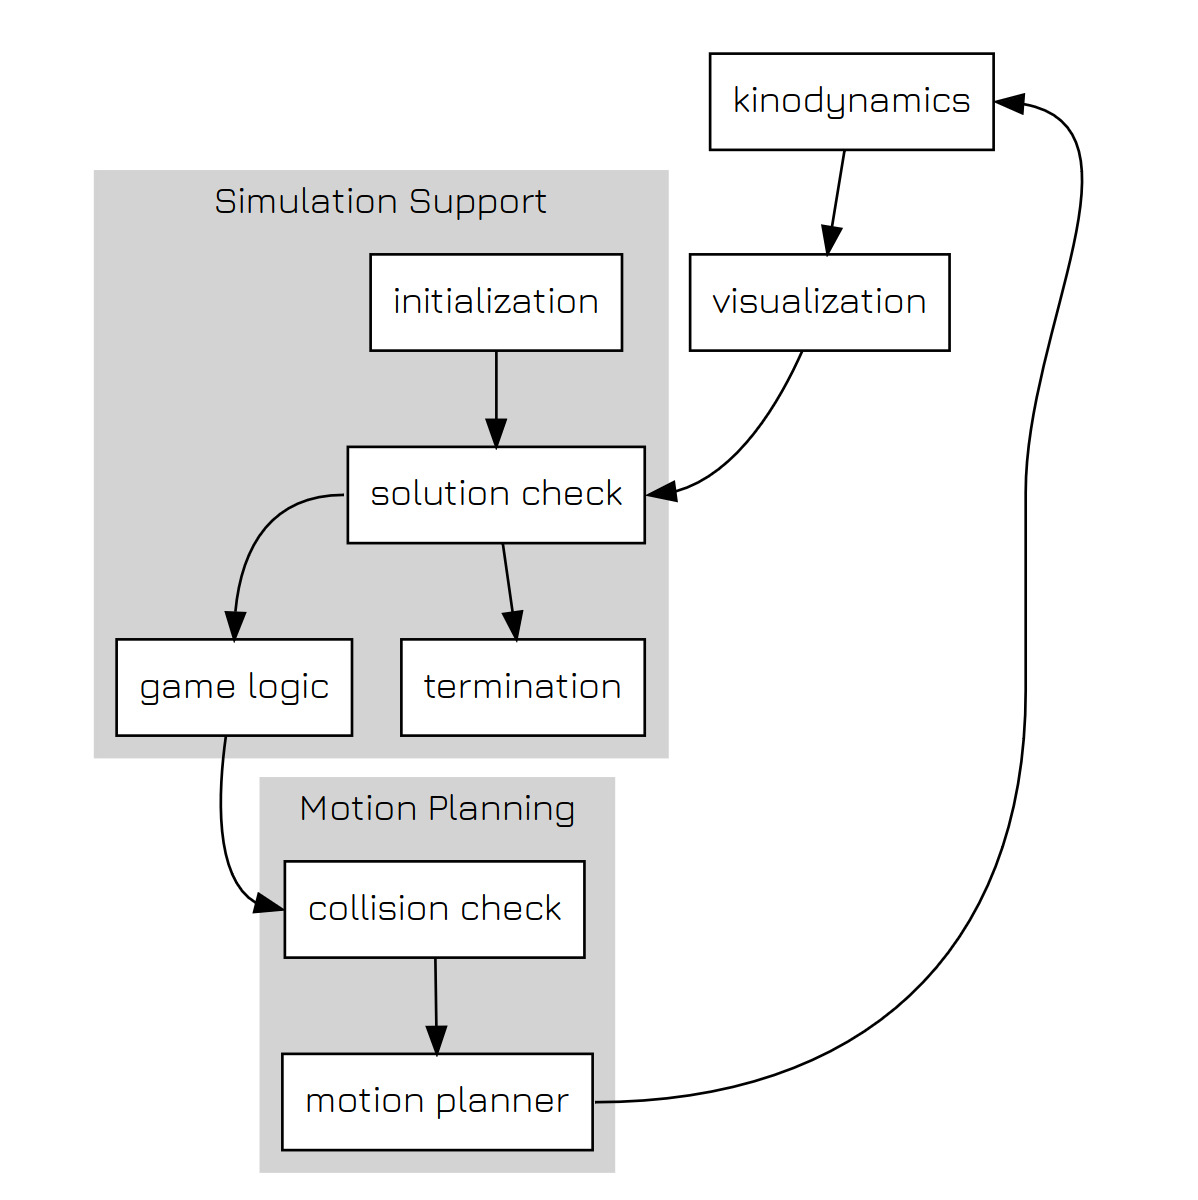
\includegraphics[width=0.5\columnwidth]{images/simulation_flowchart.jpeg}
\end{center}
\caption{Simulation structure}
\label{fig:simulation_flowchart}
\end{figure}



As shown in Fig. following points are considered in this project.

Initialization: Initial robot state along with the Initial simulation states ie. obstacle positions were set.\par
Solution Check: Robot position at goal location and termination condition such as reaching to goal location or path not found were checked.\par
Game logic: Is not used as only statis obstacles are considered in this project.\par
Collision Checking: Collisions given the current robot configuration and world state were considered for collision free path planning.\par
Motion Planning: Motion planner is implemented using current robot state as input and trajectory fro robot controller was calculated.\par
Kinodynamics: Considering the the different steering mechanisms which commands for specific kinematics constraints and dynamic equations were considered in deciding the algorithm. \par
Visualization: Animation frames for each iteration were created using simplified graphics in Matplotlib as well as 3D visualization in Gazebo.\par

Simulation initialization stage images are shown below.

\begin{figure}[htbp!]
\begin{center}
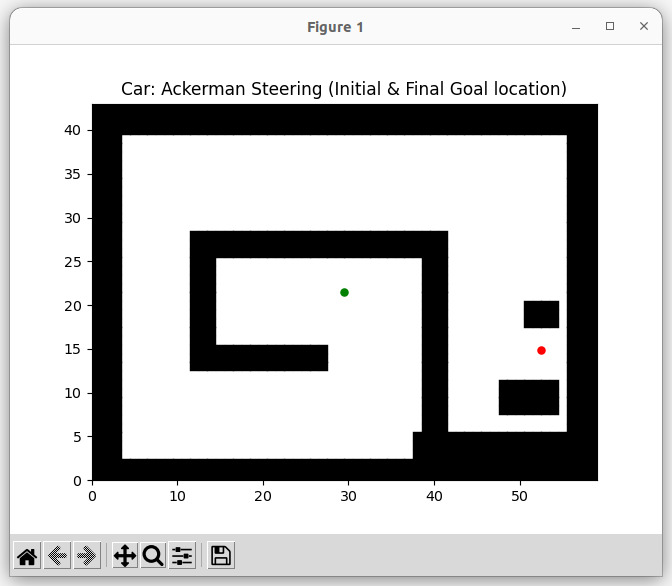
\includegraphics[width=0.6\columnwidth]{images/Car_state_initialization.jpeg}\par \vspace{3mm}
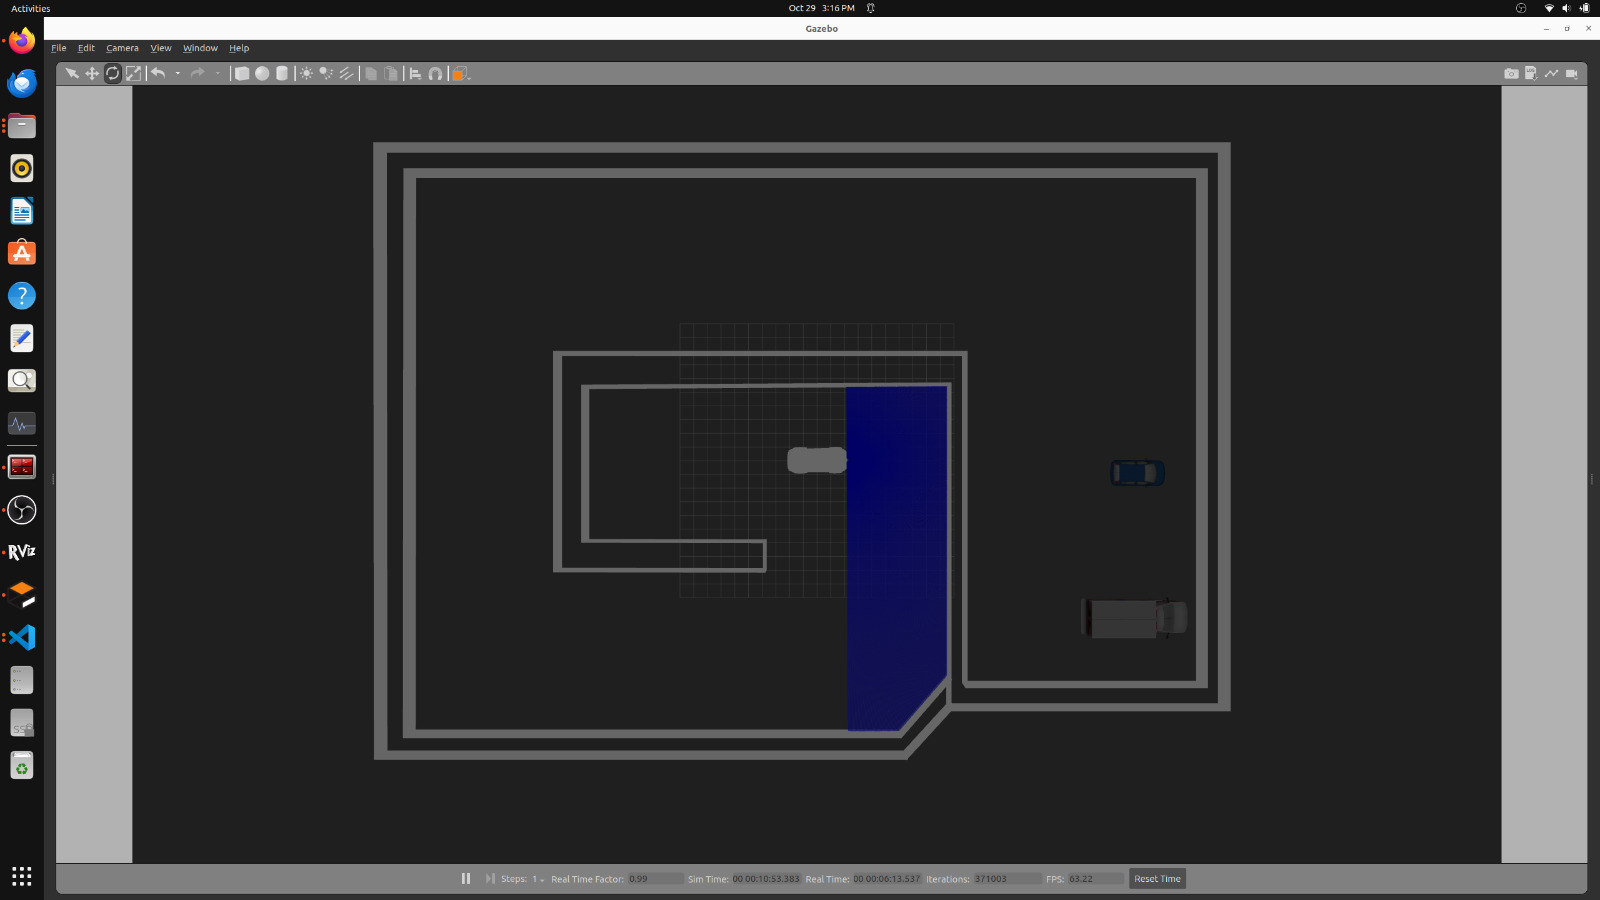
\includegraphics[width=0.6\columnwidth]{images/Gazebo_states_initialization.jpeg}\par
\vspace{3mm}
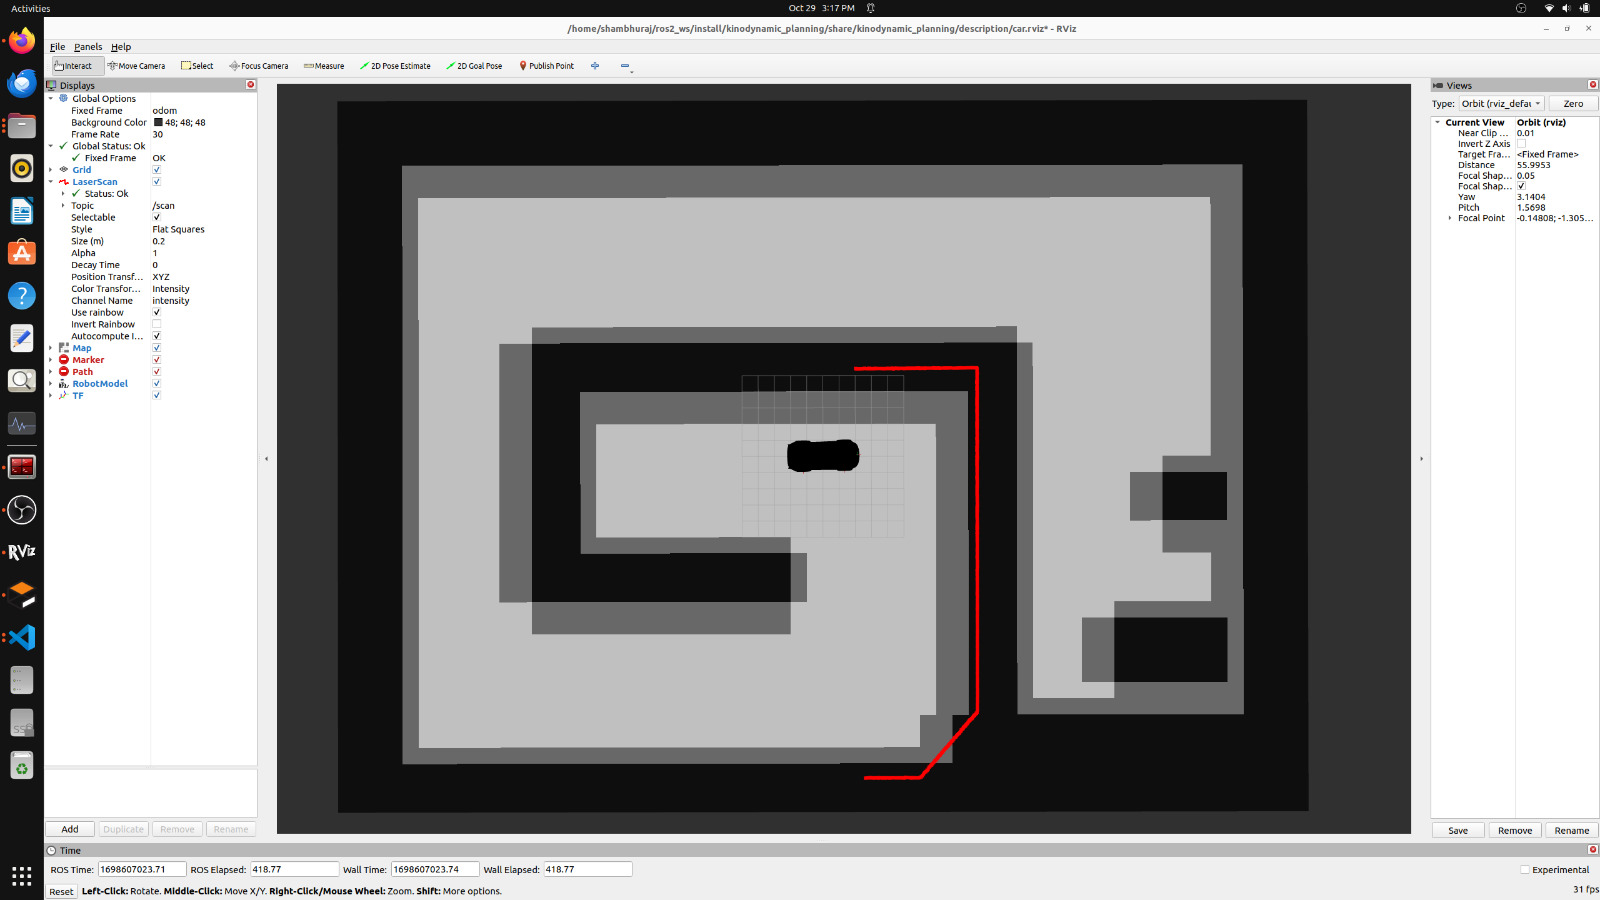
\includegraphics[width=0.6\columnwidth]{images/Rviz_state_initialization.jpeg}
\end{center}
\caption{Simulation Environment in matplotlib, Gazebo and Rviz}
\label{fig:simulation_flowchart}
\end{figure}


\subsection{Collision Checking}\label{sec:Collision Checking} \par


As shown in Fig. the environment is divided into Occupancy grid.
Occupancy grids allow you to represent the environment as a grid where each cell indicates whether it is occupied by an obstacle or free space. This representation is particularly useful for motion planning because it provides a structured way to model the environment's obstacles and free areas. A module scipy.spatial.KDTree in Python Scipy is used in this project. \par
Using a KD-Tree for occupancy grid data can be beneficial for tasks such as nearest-neighbor search, collision checking, or other spatial queries. KD-Trees are a data structure that can efficiently partition and organize your occupancy grid data.\par

Occupancy grids have advantages like, well suited for discrete planners, low storage/memory requirements and tree can be utilized for better space and computational efficiency\par

\begin{figure}[h!]
\begin{center}
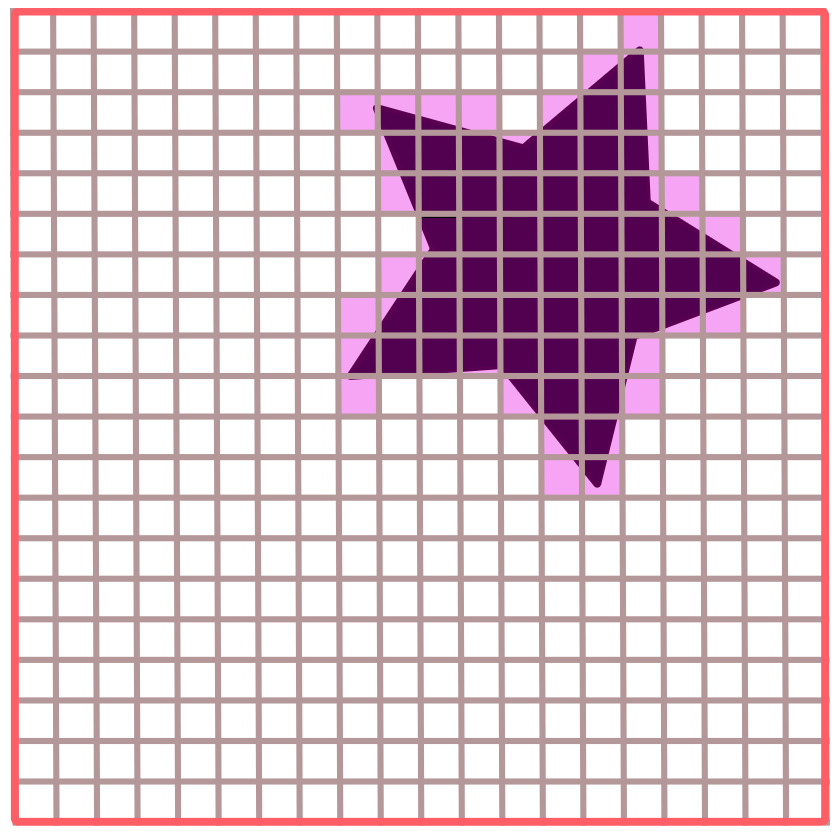
\includegraphics[width=0.5\columnwidth]{images/occupancy_grid.jpeg}
\end{center}
\caption{Occupancy grid}
\label{fig:Occupancy_grid}
\end{figure}\par


\subsection{Discrete Motion Planning with Nonholonomic Constraints}\label{sec:kinematic constraints} \par

For static planners the C-space representation is sufficient which takes into account robot's position and orientation. State space (X) incorporates the dynamic state and extend C-space by including time derivative of each dimension in the C-space. 
Working in state space allows planner to incorporate dynamic constraints on path doubles the dimensionality of the planning problem. Holonomic and non-holonomic constraints are concepts used in the field of mechanics and robotics to describe the constraints on the motion of objects or systems. Planners must incorporate robot dynamics and model the relationship between control inputs and state. These constraints may vary based on the specific vehicle configuration.
\begin{itemize}
    \item Modeling of Delivery robot: Differential drive/skid steering \par
        \begin{figure}[htbp!]
        \begin{center}
        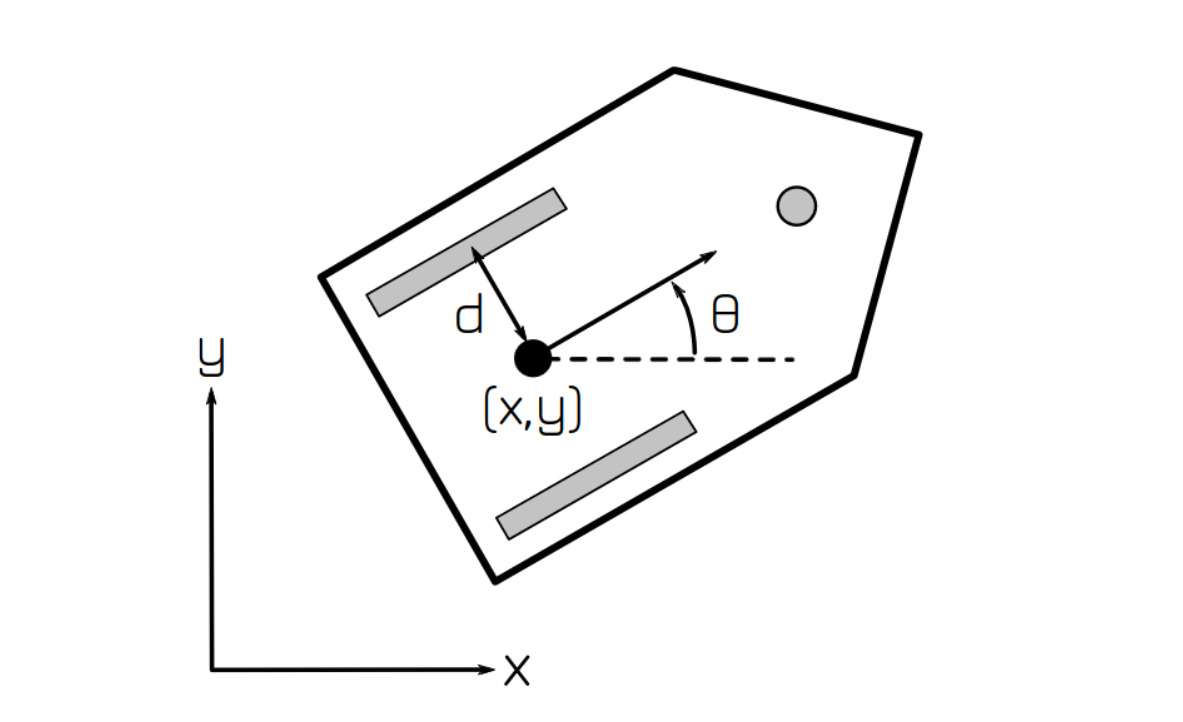
\includegraphics[width=0.4\columnwidth]{images/model_diffdrive.jpeg}         
        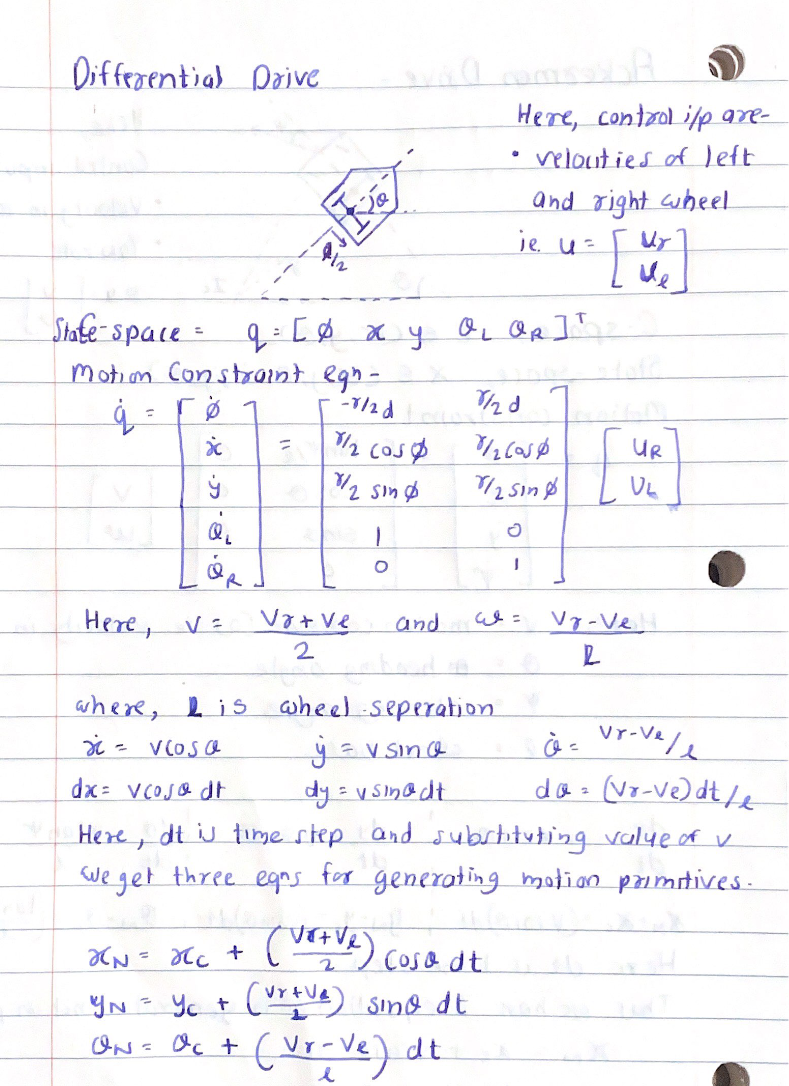
\includegraphics[width=0.4\columnwidth]{algorithm/diffbot_model.png}
        \end{center}
        \caption{Modeling of Delivery robot: Differential drive/skid steering}
        \label{fig:model_diffdrive}
        \end{figure}
        Equations for modeling differential drive robot are shown in Fig.\par
        Car class was used to define the dimension of the car in algorithm for given car model simulated in Gazebo environment.
        \par
        class  DiffBot:       \par
            speedPrecision = 4\par
            wheelSeperation=0.287 * 5          \par
            botDiameter=0.32 * 5 \par
            wheelDiameter=0.066 *5\par
            maxVelocity=2.0\par
            minVelocity=1.0\par
            stepSize=0.5\par
        Calculations using these equations are shown below:

        
    \item Modeling of Car: Ackermann steering
        \begin{figure}[htbp!]
        \begin{center}
        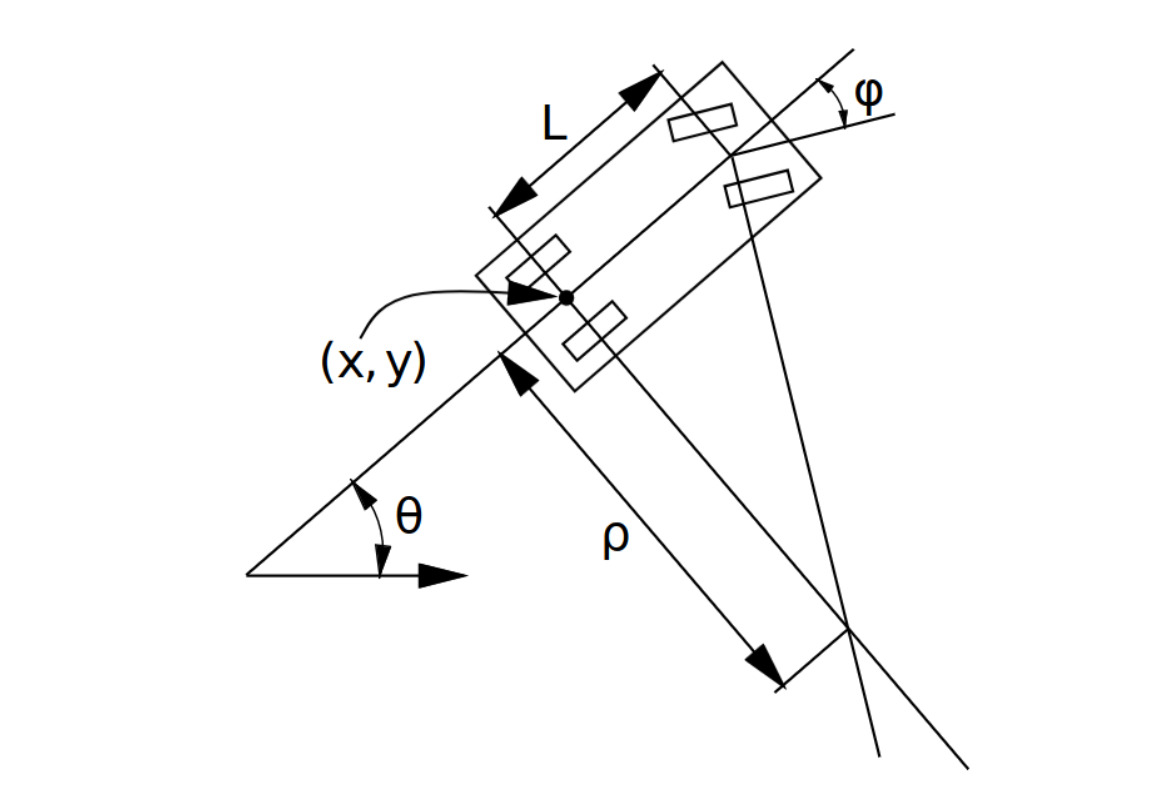
\includegraphics[width=0.4\columnwidth]{images/model_car.jpeg}
        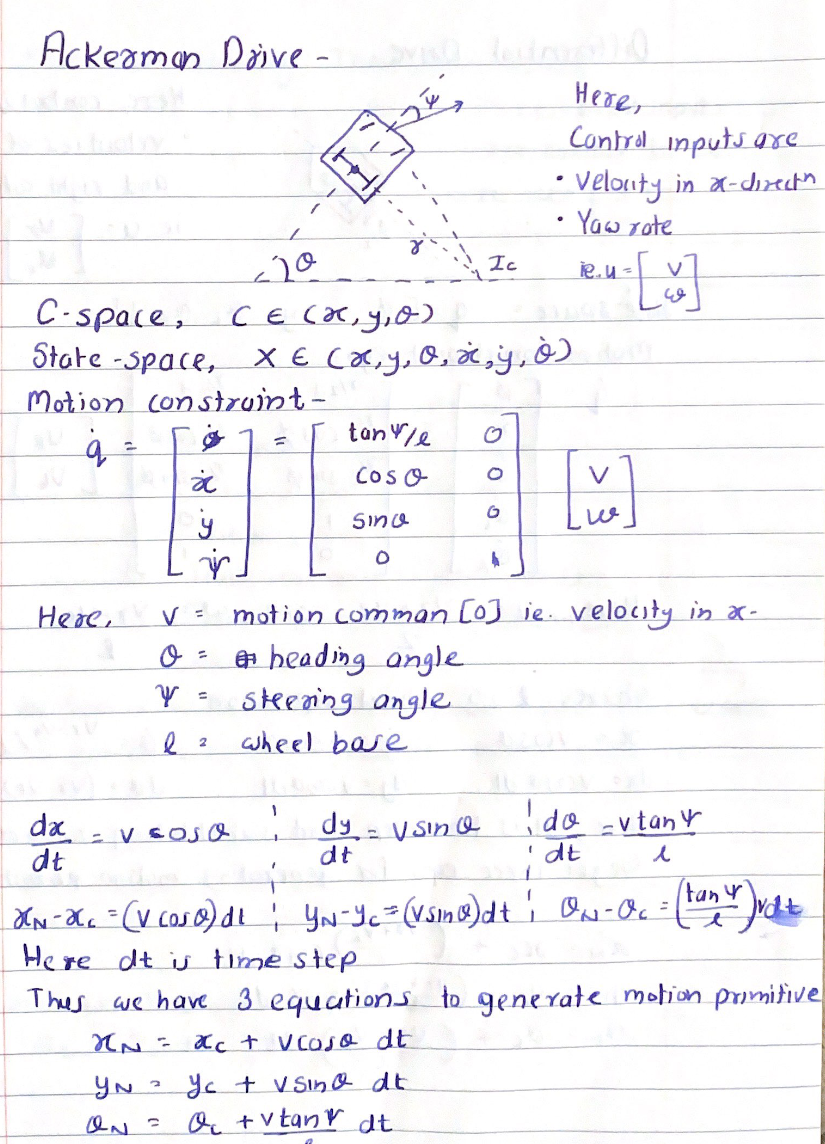
\includegraphics[width=0.4\columnwidth]{algorithm/car_model.png}
        \end{center}
        \caption{Modeling of Car: Ackermann steering}
        \label{fig:Occupancy_grid}
        \end{figure}
        Equations for modeling differential drive robot are shown in Fig.\par
        Car class was used to define the dimension of the car in algorithm for given car model simulated in Gazebo environment.
        \par
        class Car:\par
            maxSteerAngle = 0.6\par
            steerPresion = 5\par
            wheelBase = 2.58\par
            axleToFront = 3.0\par
            axleToBack = 0.4\par
            width = 2.0\par
        Calculations using these equations are shown below:
      
        
    \item Modeling of Truck with trailer: \par 
        \begin{figure}[htbp!]
        \begin{center}
        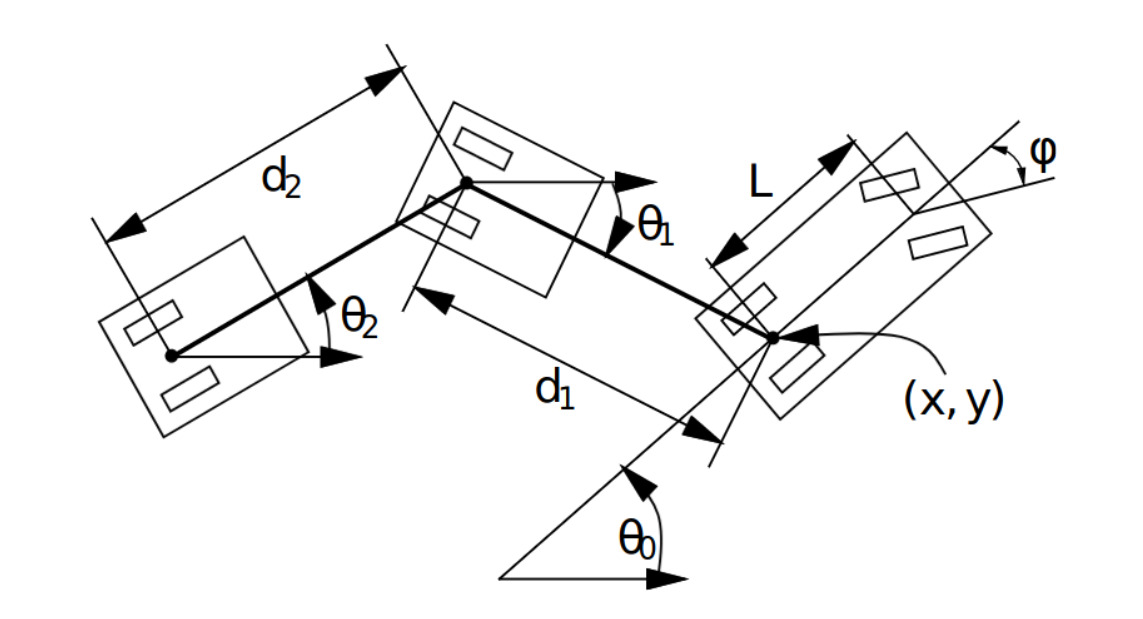
\includegraphics[width=0.4\columnwidth]{images/model_trailer.jpeg}
        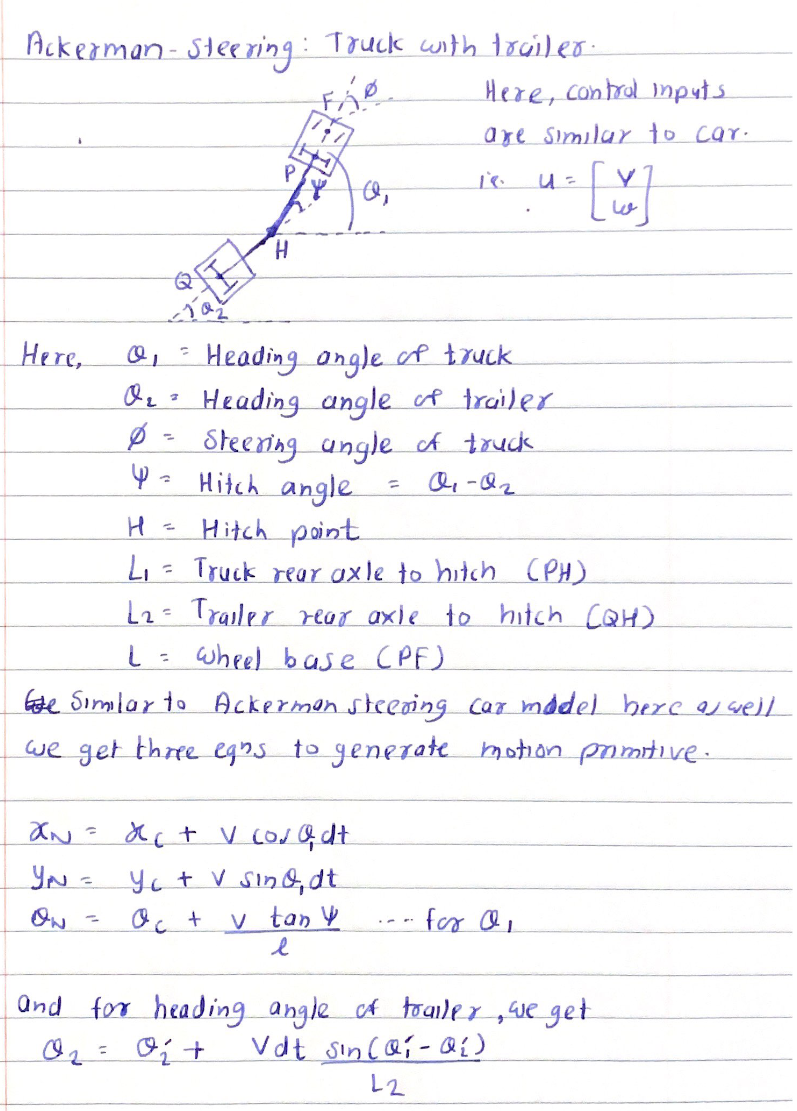
\includegraphics[width=0.4\columnwidth]{algorithm/truck_model.png}
        \end{center}
        \caption{Modeling of Truck with trailer}
        \label{fig:Occupancy_grid}
        \end{figure}
        Ackermann steering plus trailer kinematics Equations for modeling differential drive robot are shown in Fig.\par
        Car class was used to define the dimension of the car in algorithm for given car model simulated in Gazebo environment.
        \par
        class CarWithTrailer:\par
            maxSteerAngle = 0.6\par
            steerPresion = 10\par
            wheelBase = 2.58    [m] wheel base: rear to front steer\par
            axleToFront = 3.0   [m] distance from rear to vehicle front end of vehicle\par
            axleToHitch = 0.4   \par
            hitchToTrailer = 2.0\par
            axleToBack = 0.4     [m] distance from rear to vehicle back end of vehicle\par
            width = 2.0    [m] width of vehicle\par
            RTF = 0.4   [m] distance from rear to vehicle front end of trailer\par
            RTB = 4.0   [m] distance from rear to vehicle back end of trailer\par
        Calculations using these equations are shown below:\par

\end{itemize}


\subsection{Hybrid A-star algorithm}\label{sec:Hybrid A-star algorithm} \par


The Hybrid A* algorithm is a motion planning algorithm used in robotics to find collision-free paths for vehicles or robots with non-holonomic constraints, such as cars. It combines elements of both continuous and discrete state spaces, providing a compromise between computational efficiency and precision in path planning. \par
The algorithm is as follows:

\begin{figure}[h!]
\begin{center}
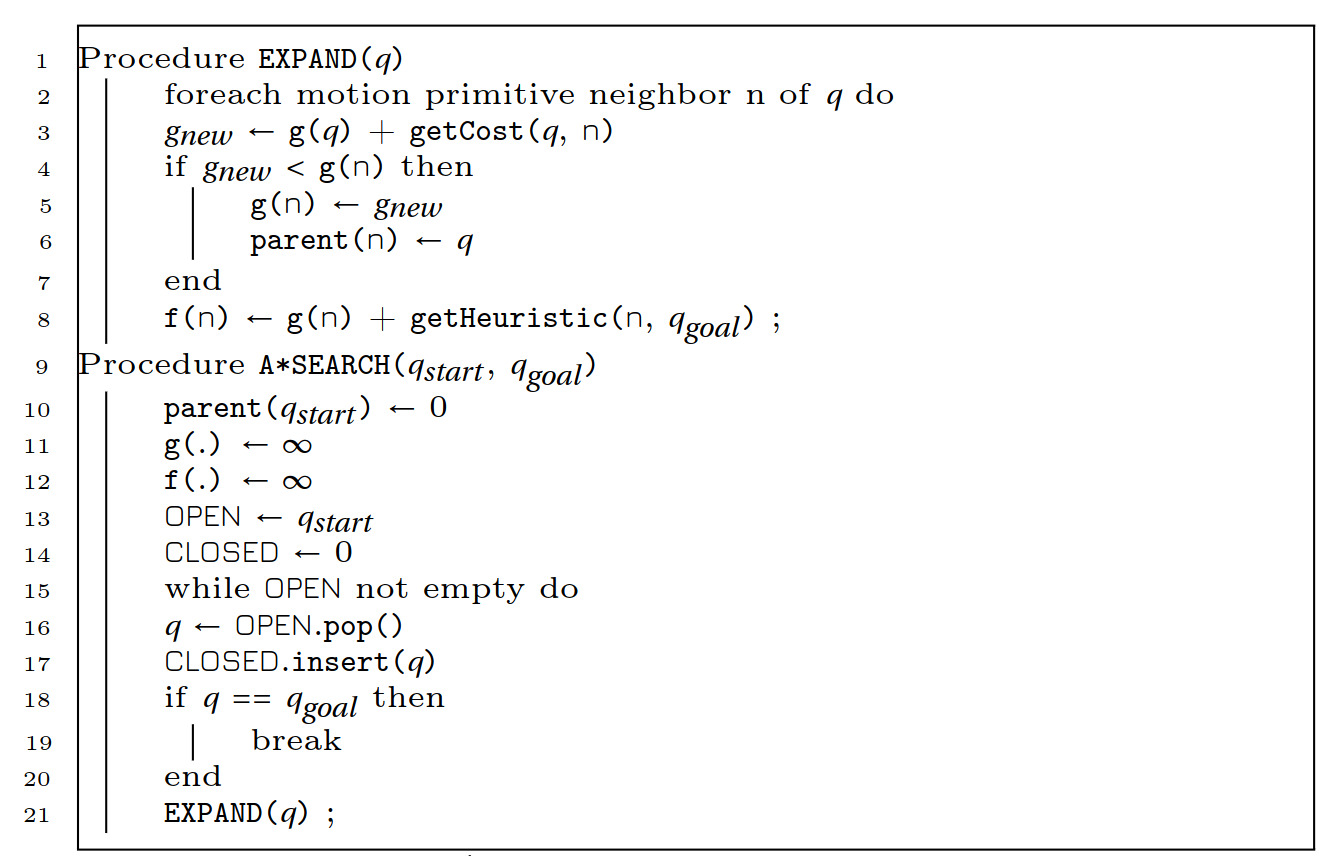
\includegraphics[width=1.0\columnwidth]{images/astar.jpeg}
\end{center}
\caption{Hybrid A-star algorithm}
\label{fig:Hybrid_A-star}
\end{figure}



\par
Following is the code for hybrid A star algorithm used for this project.
\begin{itemize}
    \item Model and cost initialization for each vehicle. \par

 
        \begin{figure}[h!]
        \begin{center}
        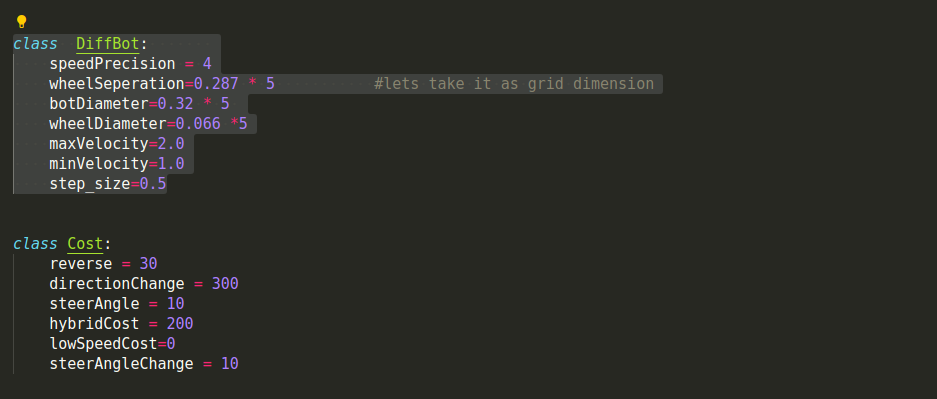
\includegraphics[width=0.8\columnwidth]{algorithm/diff_model_cost_initialization.png}
        \end{center}
        \caption{Model and cost initialization for Differential robot}
        \label{fig:Hybrid_A-star}
        \end{figure}

        \begin{figure}[h!]
        \begin{center}
        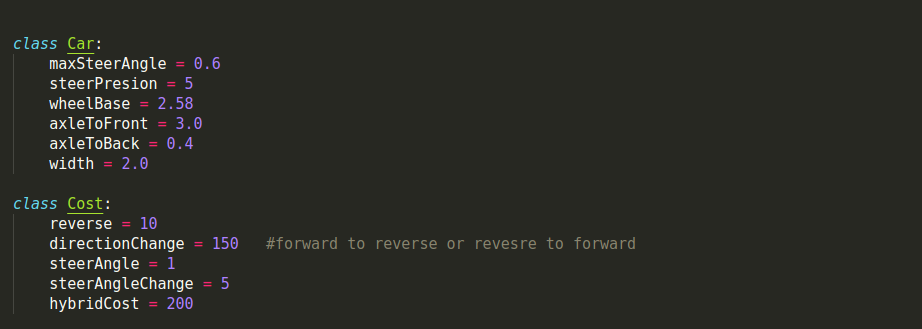
\includegraphics[width=0.8\columnwidth]{algorithm/car_model_cost_initialization.png}
        \end{center}
        \caption{Model and cost initialization for car}
        \label{fig:Hybrid_A-star}
        \end{figure}

        \begin{figure}[h!]
        \begin{center}
        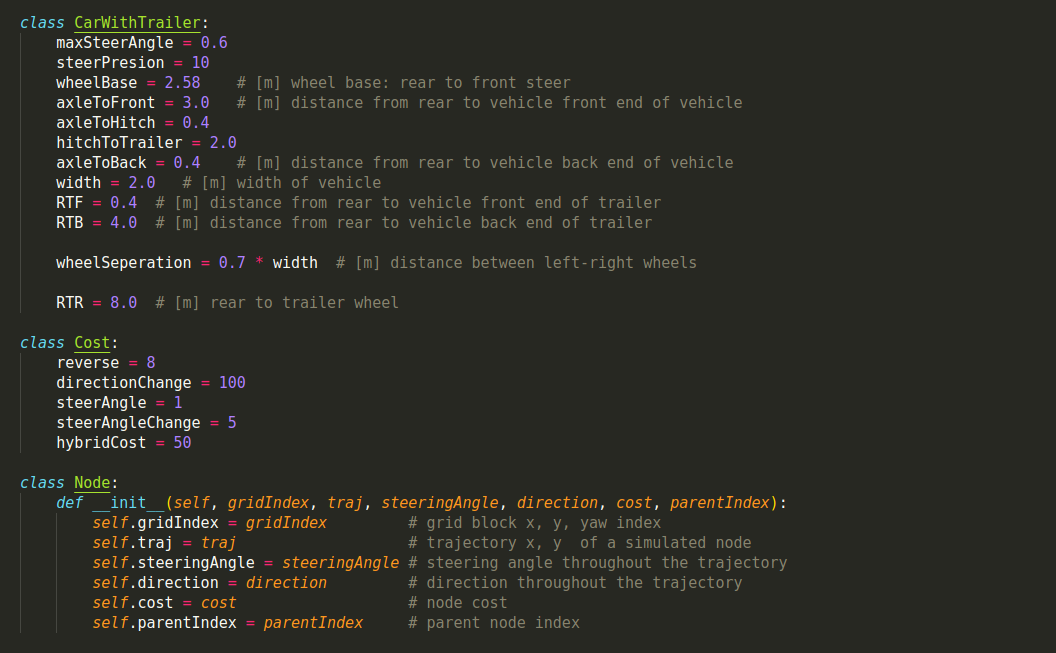
\includegraphics[width=0.8\columnwidth]{algorithm/trailer_model_cost_initialization.png}
        \end{center}
        \caption{Model and cost initialization for truck with trailer}
        \label{fig:Hybrid_A-star}
        \end{figure}

    \item Initialization of hybrid A star algorithm
        \begin{figure}[h!]
        \begin{center}
        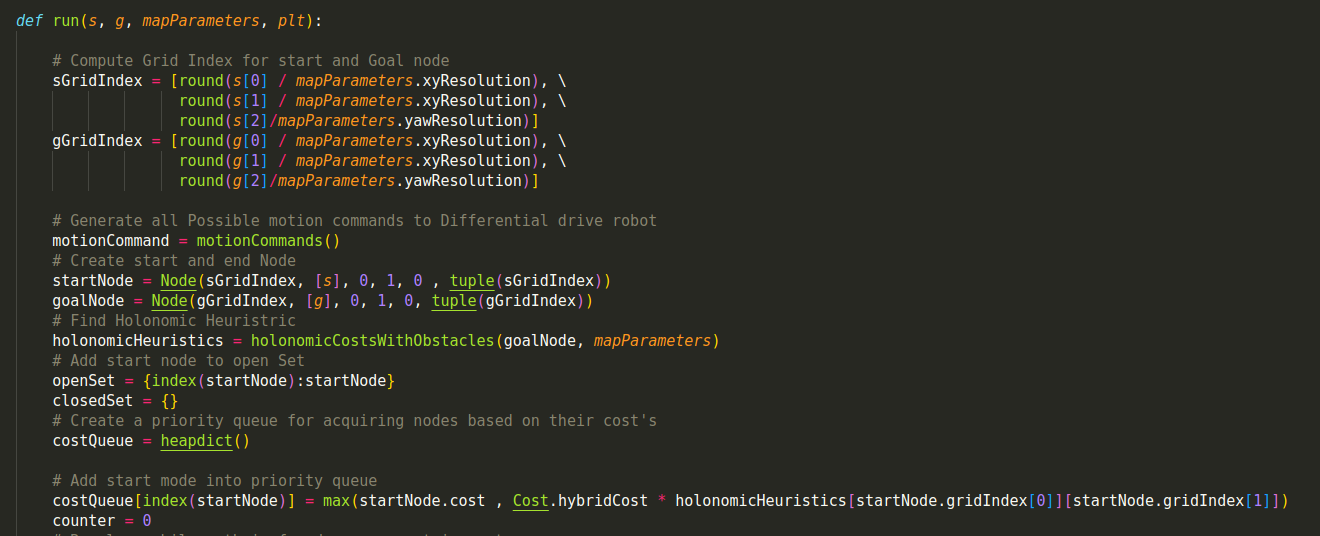
\includegraphics[width=0.8\columnwidth]{algorithm/initialization.png}
        \end{center}
        \caption{Initialization of hybrid A star algorithm}
        \label{fig:Hybrid_A-star}
        \end{figure}
    \item While loop for Hybrid A star
        \begin{figure}[h!]
        \begin{center}
        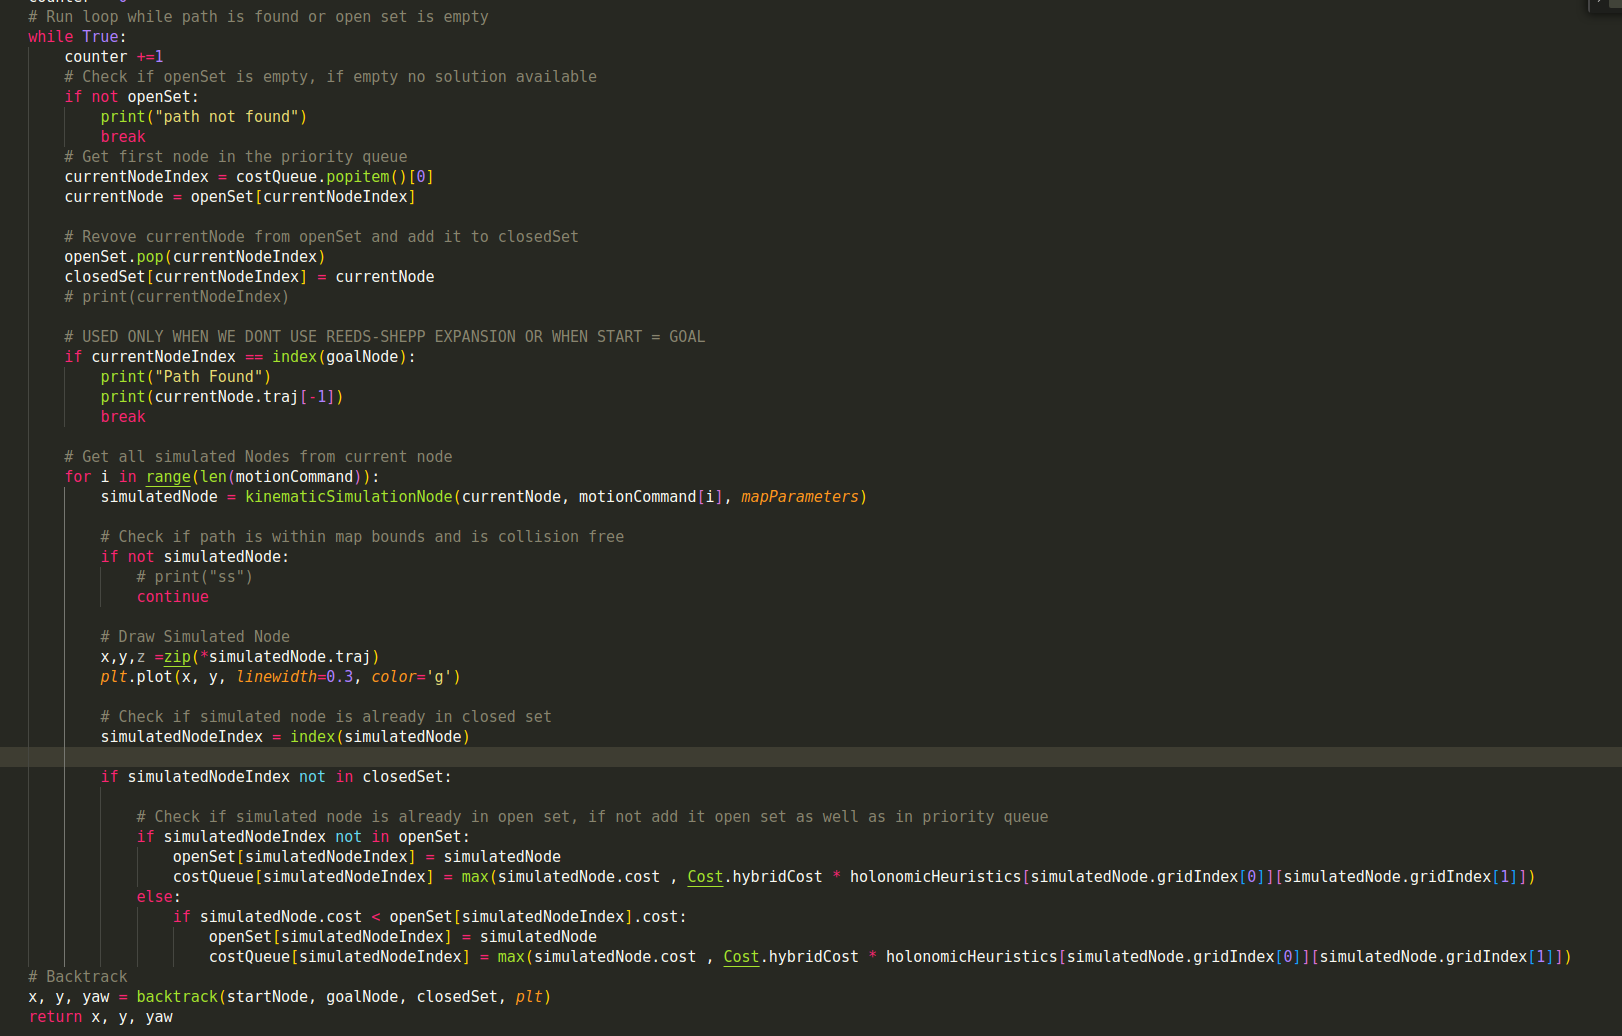
\includegraphics[width=0.8\columnwidth]{algorithm/while_loop.png}
        \end{center}
        \caption{While loop for Hybrid A star}
        \label{fig:Hybrid_A-star}
        \end{figure}
    \item Calculating holonomic cost considering obstacles
        \begin{figure}[h!]
        \begin{center}
        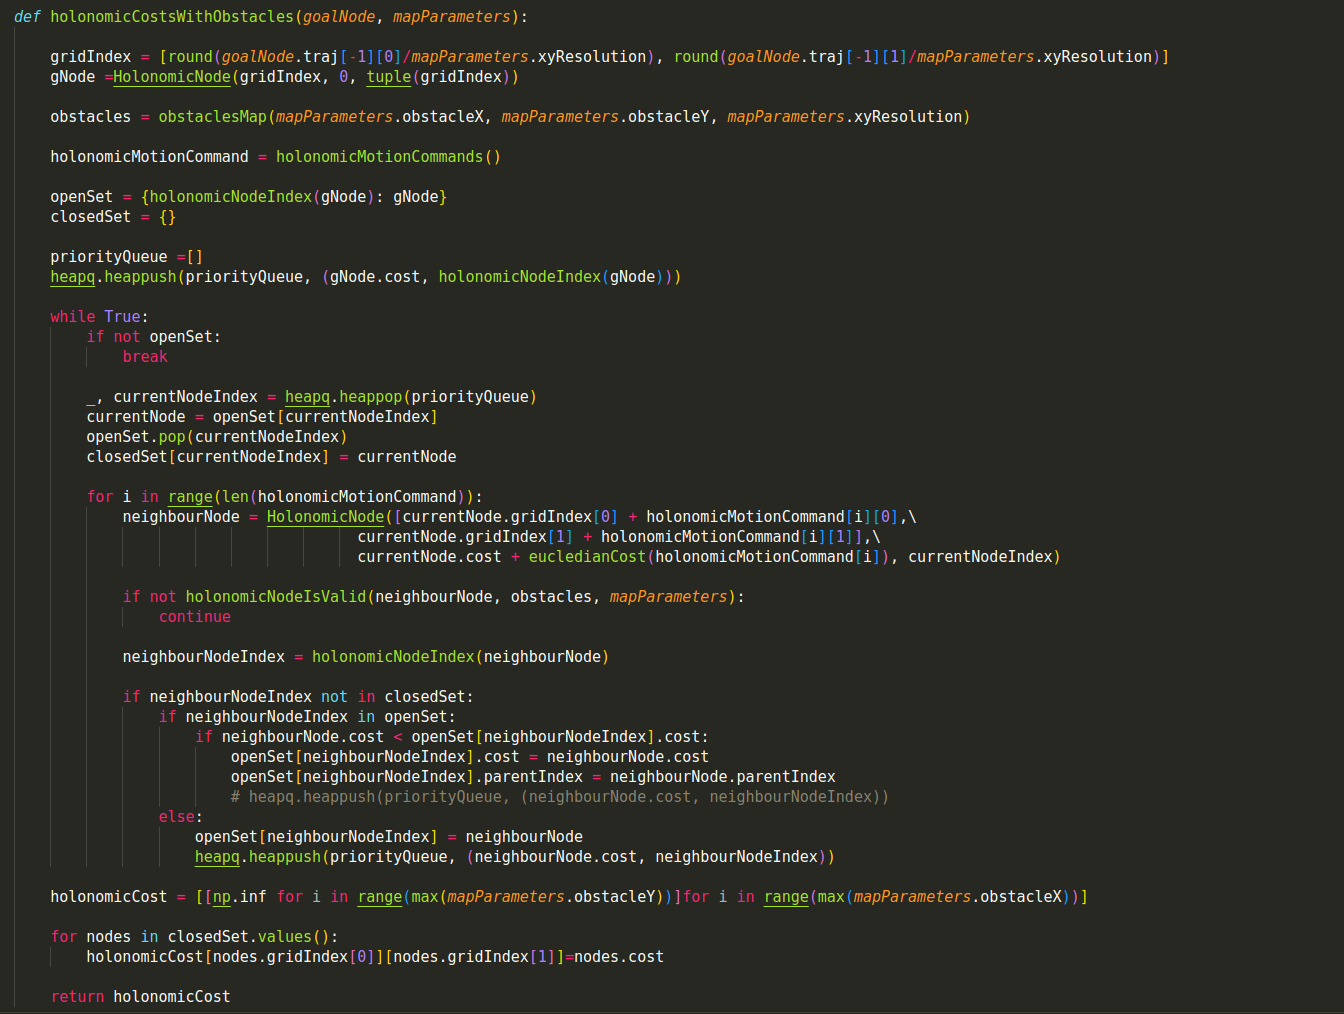
\includegraphics[width=0.8\columnwidth]{algorithm/heuristic_cost.png}
        \end{center}
        \caption{Calculating holonomic cost considering obstacles}
        \label{fig:Hybrid_A-star}
        \end{figure}
    \item Holonomic node validity check (map bounds and collision)
        \begin{figure}[h!]
        \begin{center}
        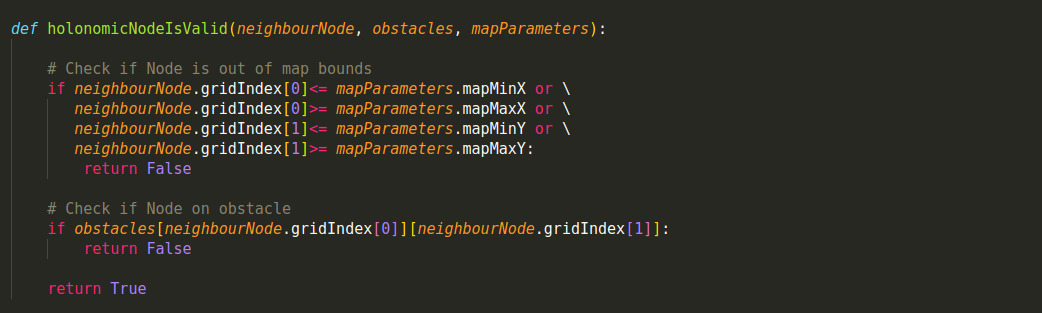
\includegraphics[width=0.8\columnwidth]{algorithm/holonomic_validation.jpeg}
        \end{center}
        \caption{Holonomic node validity check (map bounds and collision)}
        \label{fig:Hybrid_A-star}
        \end{figure}
    \item Motion commands for Differential robot
        \begin{figure}[h!]
        \begin{center}
        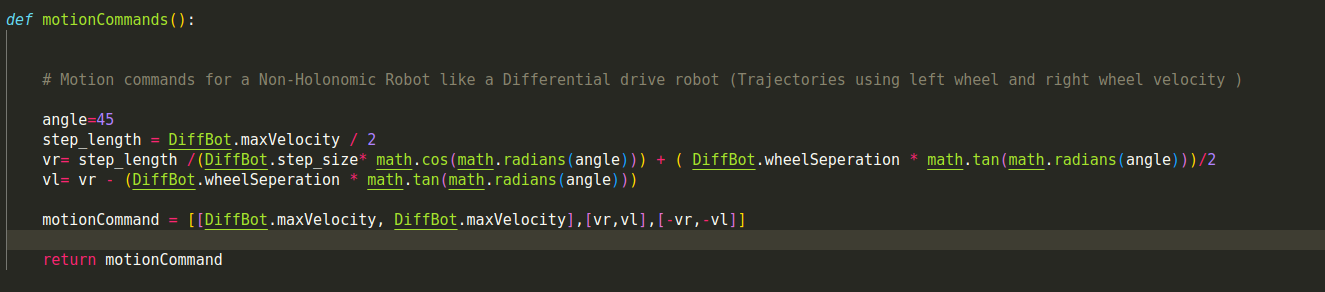
\includegraphics[width=0.8\columnwidth]{algorithm/diff_motion_command.png}
        \end{center}
        \caption{Motion commands for Differential robot}
        \label{fig:Hybrid_A-star}
        \end{figure}
    \item Simulating kinematic motion (Motion primitive)
        \begin{figure}[h!]
        \begin{center}
        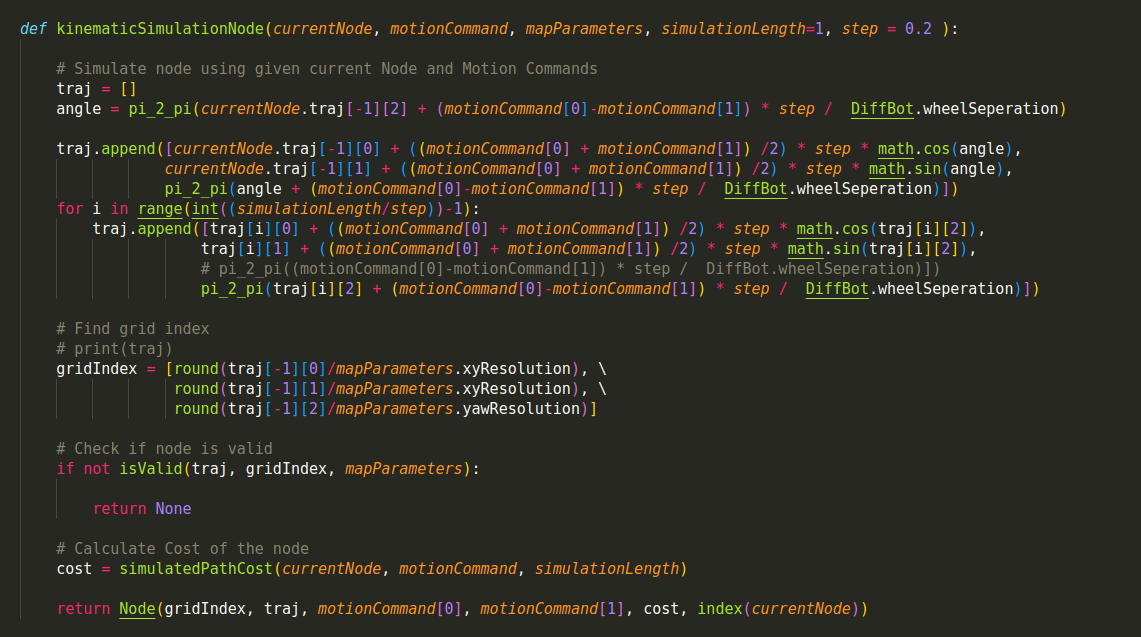
\includegraphics[width=0.8\columnwidth]{algorithm/motion_prmitive.png}
        \end{center}
        \caption{Simulating kinematic motion (Motion primitive)}
        \label{fig:Hybrid_A-star}
        \end{figure}
    \item Collision check of simulated node
        \begin{figure}[h!]
        \begin{center}
        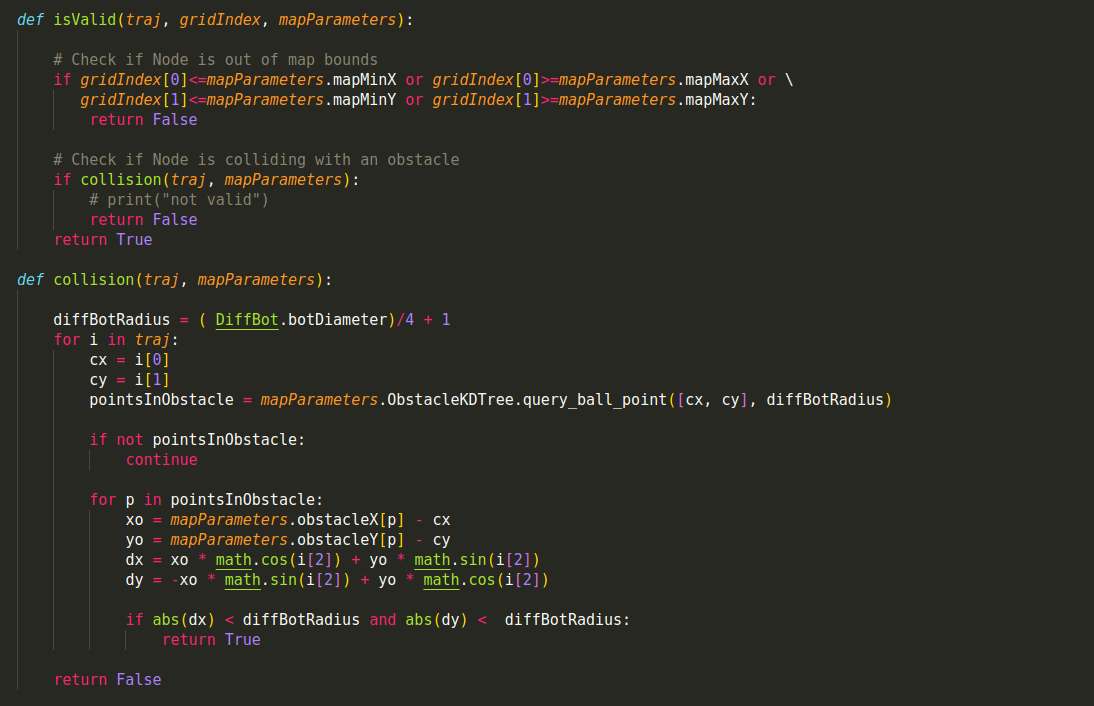
\includegraphics[width=0.8\columnwidth]{algorithm/collision_check.png}
        \end{center}
        \caption{Collision check of simulated node}
        \label{fig:Hybrid_A-star}
        \end{figure}
    \item Simulated path cost
        \begin{figure}[h!]
        \begin{center}
        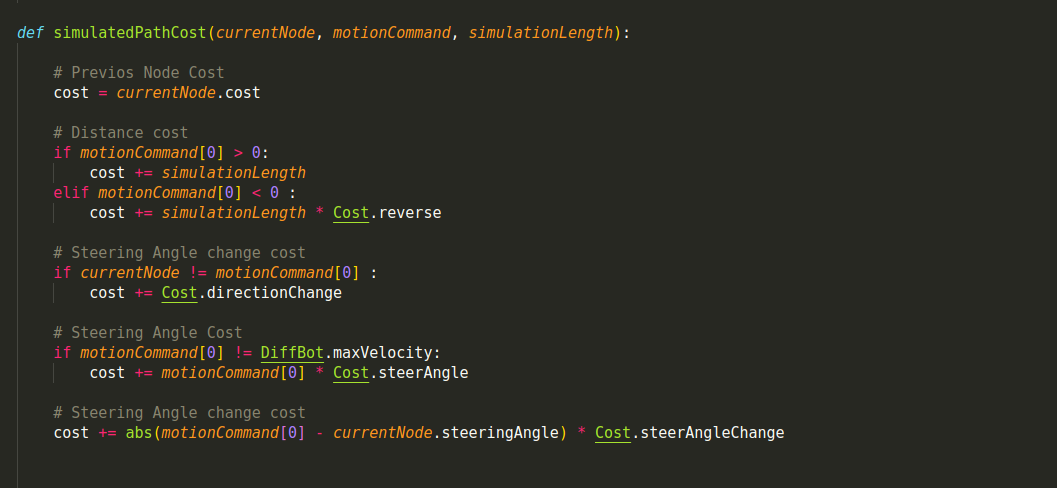
\includegraphics[width=0.8\columnwidth]{algorithm/simulation_cost.png}
        \end{center}
        \caption{Simulated path cost}
        \label{fig:Hybrid_A-star}
        \end{figure}
    \item Backtrack the lowest cost path 
        \begin{figure}[h!]
        \begin{center}
        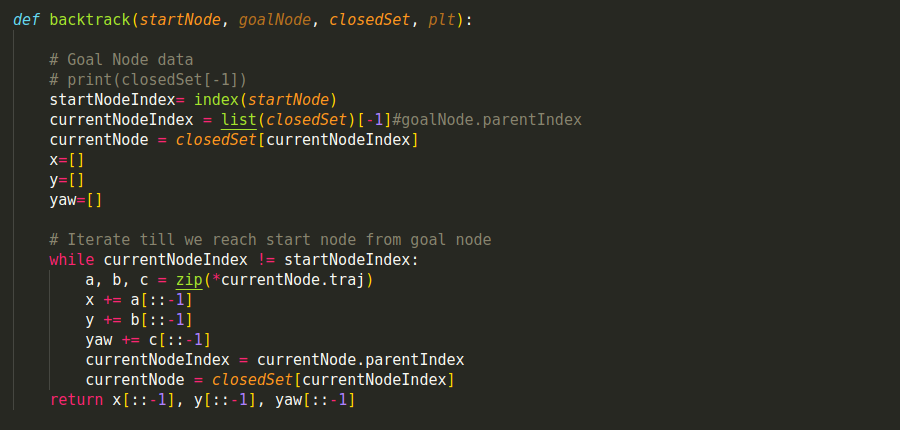
\includegraphics[width=0.8\columnwidth]{algorithm/backtrack.png}
        \end{center}
        \caption{Backtrack the lowest cost path }
        \label{fig:Hybrid_A-star}
        \end{figure}
\end{itemize}

\par





\end{document}